\chapter{Vergleich von Reaktionsmechanismen}
    Wie in Kapitel \ref{sec:reaktionsmechanismen_literatur} beschrieben, existiert eine Vielzahl von Reaktionsmechanismen, die sich hinsichtlich ihres Detaillierungsgrads und der Anzahl enthaltener Spezies und Elementarreaktionen deutlich unterscheiden. Die Komplexität eines Mechanismus beeinflusst maßgeblich den Bedarf der Rechenleistung und somit die Effizienz von Parameterstudien. 
    Da die meisten Reaktionsmechanismen ursprünglich für Verbrennungsprozesse entwickelt und validiert wurden, ist ein Vergleich ihrer Eignung für die Modellierung der partiellen Oxidation erforderlich. 
    \section{Überblick über die Reaktionsmechanismen}
    Als Grundlage der Modellierung chemischer Reaktionen nutzt Chemkin Datensätze für Reaktionsmechanismen. Es gibt verschiedene Datensätze, die sich in der Anzahl der Spezies sowie der Elementarreaktionen unterscheiden. In Tabelle \ref{tab:reaktionsmechanismen_überblick} sind die in dieser Arbeit genutzten Reaktionsmechanismen aufgelistet. 
    \begin{table}[H]
        \centering
        \caption{Überblick über Anzahl der Spezies sowie Reaktionen verschiedener Reaktionsmechanismen}
        \begin{tabular}{lcc}
        \toprule
        \textbf{Reaktionsmechanismus} & \textbf{Anzahl Spezies} & \textbf{Anzahl Reaktionen} \\
        \midrule
        ATR (in-house) & 28 & 112 \\
        GRI3.0         & 53 & 325 \\
        Aramco2.0      & 581 & 3037 \\
        NUIG1.1        & 2746 & 11270 \\
        CRECK *          & 159 & 2459 \\
        \bottomrule
        \end{tabular}
        \footnotesize{\\ *~bezieht sich auf den in der Arbeit verwendeten Mechanismus.}
        \label{tab:reaktionsmechanismen_überblick}
        
    \end{table}
    \subsection*{ATR}
        Der ATR-Mechanismus (in-house) stellt einen stark reduzierten Reaktionsmechanismus dar, der vor allem in komplexen Strömungssimulationen (CFD) eingesetzt wird. Aufgrund der geringen Anzahl an Spezies und Reaktionen bildet er ausschließlich die wesent\-lichen Hauptreaktionen der partiellen Oxidation von Methan bzw. Erdgas ab. Dies führt zu einer deutlich reduzierten Rechenzeit und ermöglicht den Einsatz in großskaligen Reaktornetzwerken oder gekoppelten CFD-Simulationen. Allerdings können mit diesem Mechanismus keine detaillierten chemischen Prozesse wie Nebenreaktionen, radikalische Zwischenprodukte oder Emissionspfade (z. B. NO$_x$-Bildung) erfasst werden, wodurch seine Anwendung auf vereinfachte Modellstudien beschränkt ist.
    \subsection*{GRI-Mech 3.0}
        GRI-Mech 3.0 ist ein detaillierter Reaktionsmechanismus, der ursprünglich im Rahmen des \emph{Gas Research Institute (GRI)} entwickelt wurde, um die Verbrennung von Methan und Erdgas realistisch zu beschreiben. Er umfasst 53 Spezies und 325 Elementarreaktionen und ist für die Hochtemperaturverbrennung sowie für die NO$_x$-Bildung optimiert \cite{Gri-Mech}.

        Der Mechanismus wurde umfassend anhand von Flammenexperimenten, Zündverzögerungszeiten und Emissionsmessungen validiert. In der Literatur gilt Gri-Mech oft als Referenzmechanismus und wird häufig für die Entwicklung von ROMs herangezogen. 

        Ein wesentlicher Vorteil von GRI-Mech ist sein geringer Umfang, wodurch der Mechanismus ähnlich wie ATR auch in Strömungssimulationen einsetzbar ist. Gleichzeitig enthält er ausreichend Reaktionspfade, um wichtige Phänomene korrekt nachzubilden. Einschränkungen bestehen jedoch bei höheren Kohlenwasserstoffen (ab C$_3$ - C$_4$), sowie im Niedertemperaturbereich.
    \subsection*{AramcoMech 2.0}
        Der AramcoMech 2.0 Reaktionsmechanismus ist ein Mechanismus mit einem hohen Detailgrad. Er wurde von der National University of Galway in Zusammenarbeit mit Saudi Aramco entwickelt. Dieser Mechanismus umfasst 581 Spezies und mehr als 3000 elementare Reaktionen und ist insbesondere auf die Oxidation und Verbrennung von kurzkettigen Kohlenwasserstoffen optimiert \cite{Aramco20}. 

        Der Mechanismus wurde umfassend anhand von  Zündverzögerungszeiten, laminaren Flammengeschwindigkeiten sowie Species-Profilen validiert. Dabei deckt diese einen breiten Bereich an Bedingungen ab, darunter hohe Drücke und Temperaturen. Damit ist AramcoMech 2.0 für die Simulation von technisch relevanten Verbrennungsprozessen geeignet, bei denen neben Methan auch andere Stoffe wie Ethan, Ethen, Propan und Propen eine Rolle spielen. 

        Durch den deutlich höheren Detailgrad dieses Mechanismus ist die Verwendung desselben in CFD-Simulationen sehr rechenintensiv. 
    \subsection*{NUIGMech1.1}
        NUIGMech 1.1 ist ein sehr detaillierter Reaktionsmechanismus, der über 2500 Spezies und über 11000 Elementarreaktionen umfasst. Damit zählt er zu den umfangreichsten Mechanismen für die Verbrennung und Oxidation von Kohlenwasserstoffen \cite{MARTINEZ2021401}.

        Der Mechanismus wurde in einer Vielzahl von Experimenten validiert. Abgedeckt wird ein breites Spektrum an Bedingungen, darunter hohe Temperaturen, hohe Drücke und breite Äquivalenzverhältnisse. 

        Im Gegensatz zu anderen Reaktionsmechanismen unterstützt NUIGMech 1.1 weitaus mehr Brennstoffe. Validierungen wurden unter anderem für die Oxidation von Methan und Ethan, für Erdgasgemische sowie für Propan/Propen und Propin, sowie für C$_2$-C$_6$ Alkane durchgeführt \cite{MARTINEZ2021401}. Dadurch können mit diesem Mechanismus Verbrennungen modelliert werden, bei denen komplexere Brennstoffe zum Einsatz kommen. 

        Die hohe Anzahl an Spezies und Reaktionen bringt jedoch einen erheblichen Rechenaufwand mit sich. So ist der Einsatz in CFD-Simulationen nicht praktikabel. Zudem treten bei komplexeren Reaktornetzwerken oftmals Divergenzprobleme und Instabilitäten auf.
    \subsection*{CRECK Mechanismus}
        Die Creck Modeling Group hat eine Vielzahl von Reaktionsmechanismen für verschiedene Anwendungsfälle und mit unterschiedlichem Detailgrad erstellt. Komplexe Mechanismen sind dabei für die Verbrennung von C$_1$ - C$_{16}$ Alkanen bei hohen und niedrigen Temperaturen sowie für die Bildung von NO$_x$ und Ruß verantwortlich. Ein besonderer Fokus liegt auf der Bildung von Schadstoffen sowie der Betrachtung von Aromaten im Verbrennungsprozess. Es existieren sowohl sehr kompakte (62 Elementarreaktionen), als auch sehr umfangreiche (27000 Elementarreaktionen) Mechanismen \cite{CRECK_DetailedMechanisms}.
    \section{Einfluss der Mechanismusgröße auf den Rechenaufwand}
        Die Rechenzeit bei Simulationen hängt wesentlich von der Größe des verwendeten Reaktionsmechanismus ab. Dabei bestimmen vor allem die Anzahl der chemischen Spezi\-es $N_s$ und der Elementarreaktionen $N_r$ die Komplexität der numerischen Lösung. Wie in Kapitel \ref{sec:theoretische_grundlagen} beschrieben, wird für jede Spezies eine Stoffbilanzgleichung gelöst. Somit ist die Dimension des Gleichungssystems gleich der Anzahl der im Mechanismus vorhandenen Spezies. Die Berechnung der Reaktionsraten erfolgt für jede Elementarreaktion separat auf Basis der Arrhenius-Gleichung (siehe Gleichung \ref{eq:Arrhenius}), wodurch der Aufwand zur Auswertung der rechten Seiten (RHS) in guter Näherung linear mit der Reaktionszahl $N_r$ skaliert \parencite{ChemkinTheoryManual, Niemeyer2016}.

        Wesentlich aufwändiger ist die Lösung der Differentialgleichungen. CHEMKIN verwendet hierfür implizite Integrationsverfahren (BDF, CVODE) und Newton-Verfahren für stationäre Lösungen, die in jeder Iteration ein Gleichungssystem der Dimension $N_s+1$ lösen. Im ungünstigsten Fall wächst der Rechenaufwand kubisch mit der Spezieszahl $t \sim \mathcal{O}\left(N_s^3\right)$, im besten Fall mit $t \sim \mathcal{O}\left(N_s^2\right)$ \cite{CURTIS2017312}.

        Da zwischen der Anzahl der Spezies und der Anzahl der Elementarreaktionen ein direkter Zusammenhang besteht, bewirkt eine Reduzierung der Speziesanzahl eine erhebliche Verkürzung der Laufzeit. Es ist daher von hohem Interesse, einen Reaktionsmechanismus zu wählen, der alle relevanten Spezies und Elementarreaktionen abdeckt und keine nicht relevanten Spezies enthält. %Beispielsweise wäre ein Mechanismus, der eine Vielzahl an längerkettigen Kohlenwasserstoffen berücksichtigt, \alert{keine gute Wahl für diesen Anwendungsfall.} %Wertend!
        So ist die Anwendung eines Reaktionsmechanismus für die Verbrennung von Erdgas redundant, wenn er umfangreiche Reaktionen langkettiger Kohlenwasserstoffe beschreibt. 
    % ---------- gehört in Auswertungskapitel --------------
\iffalse
    \section{Simulationen}
        \label{sec:Simulationen_reaktionsmechanismus}
        Für den Vergleich der Reaktionsmechanismen wurde die Partialoxidation in einem einfachen Reaktornetzwerk, bestehend aus einem PSR und einem PFR, modelliert. In diesem stellt der PSR die Flammzone, der PFR die Nachbrennzone dar. In Abbildung \ref{fig:rom_mechanismusvergleich} ist das Reaktornetzwerk schematisch dargestellt.\\
        \begin{figure}[htbp]
          \centering
          \tikzset{
            inletoutlet/.style={
              draw,
              rounded corners=2pt,
              fill=black!10,
              minimum height=10mm,
              minimum width=20mm,
              align=center
            },
            psr/.style={
              draw,
              circle,
              fill=blue!15,
              minimum size=12mm,
              align=center
            },
            pfr/.style={
              draw,
              rectangle,
              fill=blue!15,
              minimum height=10mm,
              minimum width=25mm,
              align=center
            },
            flow/.style={
              -{Stealth[length=2.2mm]},
              thick
            }
          }
        
          \begin{tikzpicture}[node distance=20mm, font=\small]
            % Nodes
            \node[inletoutlet] (inlet) {Inlet};
            \node[psr, right=of inlet] (psr) {PSR};
            \node[pfr, right=of psr] (pfr) {PFR};
            \node[inletoutlet, right=of pfr] (outlet) {Outlet};
        
            % Arrows
            \draw[flow] (inlet) -- (psr);
            \draw[flow] (psr) -- (pfr);
            \draw[flow] (pfr) -- (outlet);
          \end{tikzpicture}
        
          \caption{Schematische Darstellung der Prozessabfolge: Inlet → PSR → PFR → Outlet.}
          \label{fig:rom_mechanismusvergleich}
        \end{figure}
        \subsection{Simulation ohne CO$_2$}
        Über die Länge der Nachbrennzone lassen sich die Stoffmengenanteile aufteilen. In Abbildung \ref{fig:vergleich_h2_ch4_keinco2} sind beispielsweise die Stoffmengenanteile von Wasserstoff und Methan dargestellt.
        \begin{figure}[H]
            \centering
            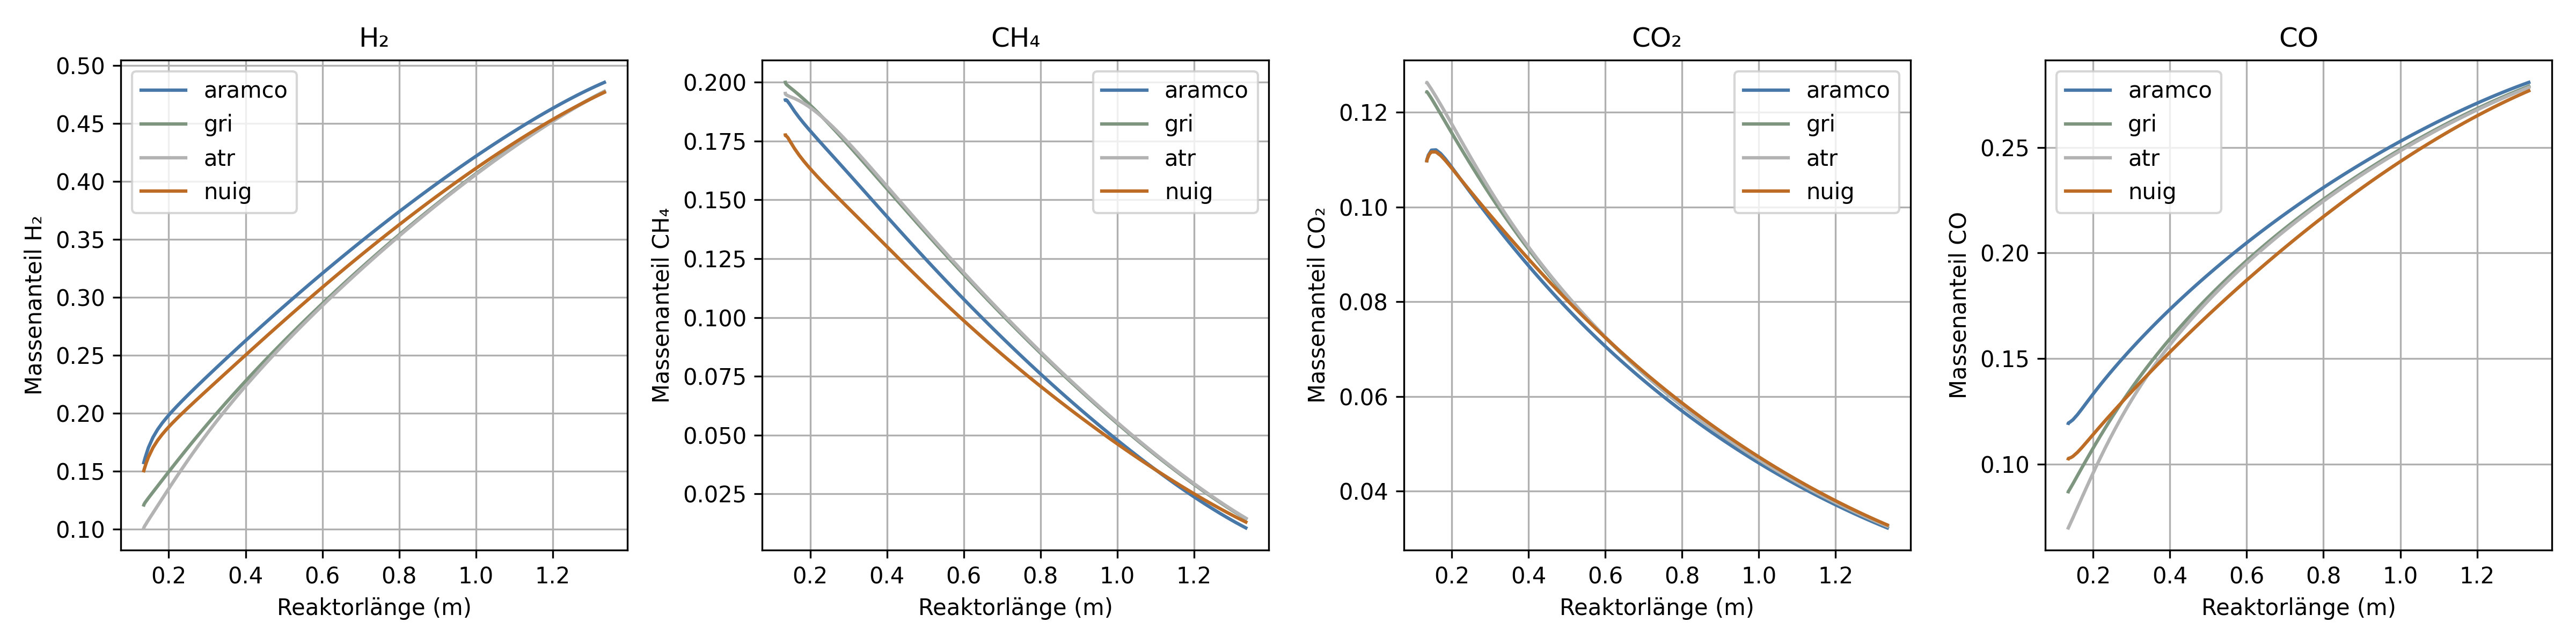
\includegraphics[width=1\linewidth]{img/Vergleich_mech/CO_CO2_keinCO2.png}
            \caption{Darstellung der Stoffmengenanteile Wasserstoff und Methan für die Simulation ohne CO$_2$}
            \label{fig:vergleich_h2_ch4_keinco2}
        \end{figure}
        Zwar zeigen sich kleine Unterschiede für die verschiedenen Reaktionsmechanismen, allerdings ähnelt sich der Verlauf immer stark. So ist die berechnete Zusammensetzung des Abgases annähernd identisch. In Tabelle \ref{tab:vergleich_abgaszusammensetzung_keinco2} sind die Ergebnisse der Simulationen sowie die experimentell vorliegenden Daten dargestellt. Dabei handelt es sich um trockengas, bei dem Wasserdampf entfernt worden ist. 
        \begin{table}[H]
            \centering
            \caption{Vergleich der Modell- und Experimentalwerte der Molenbrüche ohne CO\textsubscript{2}-Zugabe}
            \label{tab:vergleich_abgaszusammensetzung_keinco2}
            \begin{tabular}{lccccc}
                \toprule
                & \textbf{Exp.} & \textbf{GRI} & \textbf{ARAMCO} & \textbf{ATR} & \textbf{NUIG} \\
                \midrule
                \textbf{H$_2$} [Vol.-\%] & 0,599 & 0,594 & 0,600 & 0,594 & 0,596 \\
                \textbf{CO} [Vol.-\%]& 0,341 & 0,347 & 0,347 & 0,347 & 0,346 \\
                \textbf{CH$_4$} [Vol.-\%]& 0,007 & 0,018 & 0,013 & 0,018 & 0,016 \\
                \textbf{CO$_2$} [Vol.-\%]& 0,048 & 0,041 & 0,040 & 0,041 & 0,041 \\
                \bottomrule
            \end{tabular}
        \end{table}
        Die erhaltenen Werte weisen eine hohe Ähnlichkeit zu den experimentell ermittelten Werten auf, wobei es jedoch leichte Abweichungen beim Methan und Kohlenstoffdioxid gibt. 
        \subsection{Simulation mit CO$_2$}
        Analog zur Simulation ohne CO$_2$ werden die Stoffe über die Länge der Nachbrennzone analysiert (siehe Abbildung \ref{fig:vergleich_h2_ch4_co2}).
        \begin{figure}[H]
            \centering
            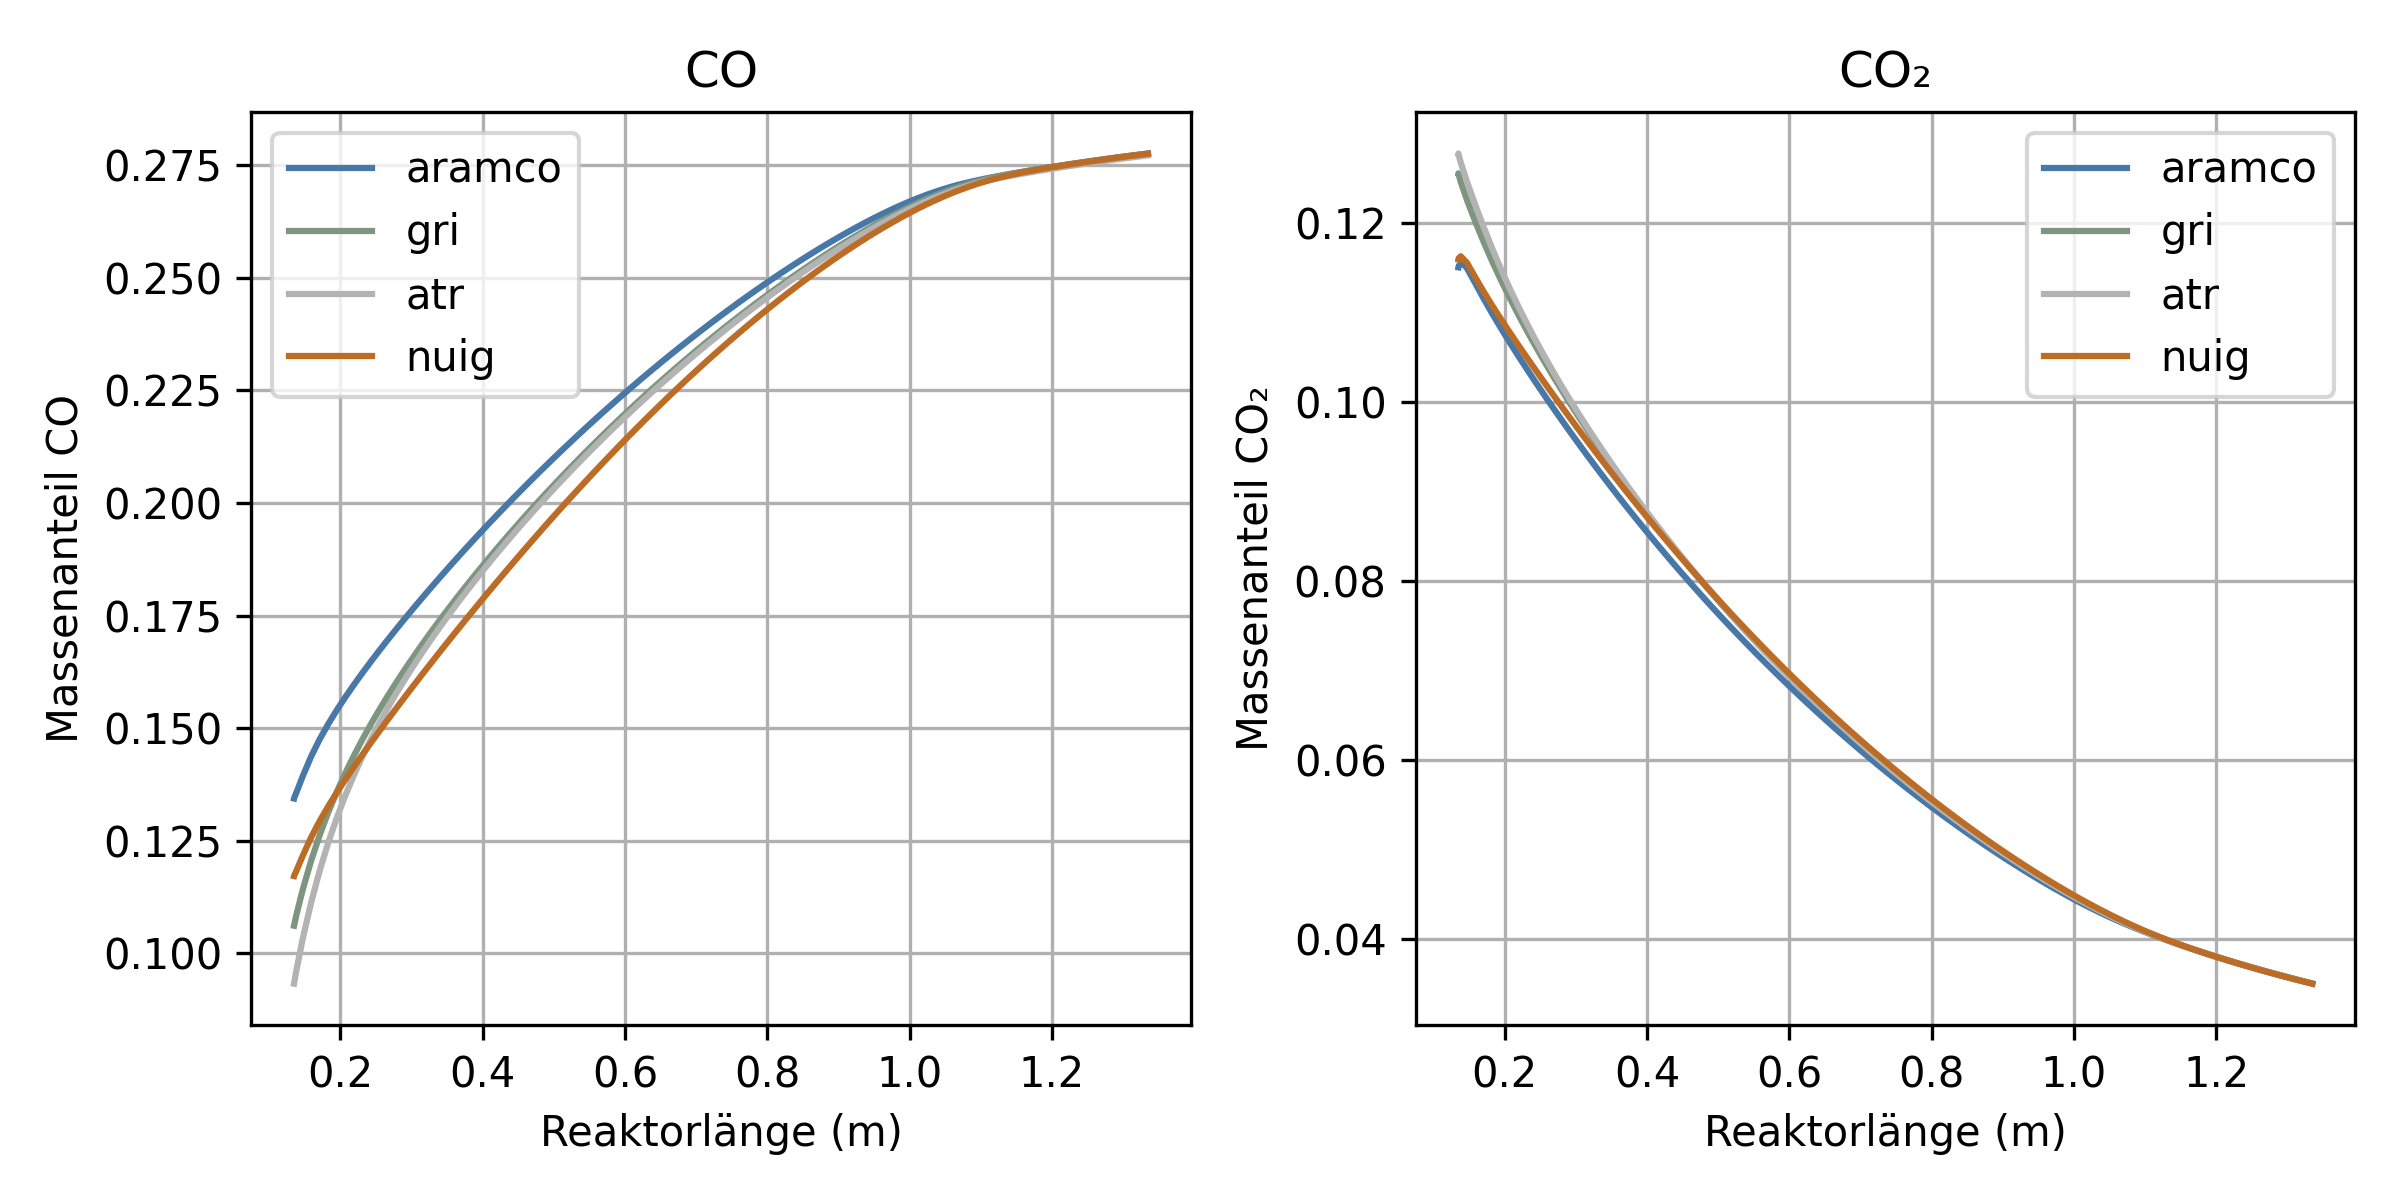
\includegraphics[width=1\linewidth]{img/Vergleich_mech/CO_CO2_CO2.png}
            \caption{Darstellung der Stoffmengenanteile Wasserstoff und Methan für die Simulation mit CO$_2$}
            \label{fig:vergleich_h2_ch4_co2}
        \end{figure}
        Auch hier zeichnet sich ein ähnliches Bild. Die Verläufe sind alle sehr ähnlich und führen zu sehr ähnlichen Abgaszusammensetzungen. In Tabelle sind die berechneten Stoffmengenanteile sowie die experimentell ermittelten Daten dargestellt (wie in Tabelle \ref{tab:vergleich_abgaszusammensetzung_keinco2}).
        \begin{table}[H]
            \centering
            \caption{Vergleich der Modell- und Experimentalwerte der Molenbrüche mit CO\textsubscript{2}-Zugabe}
            \begin{tabular}{lccccc}
                \toprule
                & \textbf{Exp.} & \textbf{GRI} & \textbf{ARAMCO} & \textbf{ATR} & \textbf{NUIG} \\
                \midrule
                \textbf{H$_2$} [Vol.-\%]& 0,416 & 0,579 & 0,579 & 0,580 & 0,579 \\
                \textbf{CO} [Vol.-\%]& 0,424 & 0,373 & 0,373 & 0,373 & 0,373 \\
                \textbf{CH$_4$} [Vol.-\%]& 0,001 & 0,000 & 0,000 & 0,000 & 0,000 \\
                \textbf{CO$_2$} [Vol.-\%]& 0,151 & 0,047 & 0,047 & 0,047 & 0,047 \\
                \bottomrule
            \end{tabular}
        \end{table}
        Im Vergleich zu den Ergebnissen der Simulation ohne Zugabe von Kohlenstoffdioxid weisen die simulierten Werte eine hohe Abweichung auf. Jedoch ergeben sich für alle Reaktionsmechanismen die gleichen Werte. \alert{Systematischer Fehler!}
\fi 